\chapter{RESULT ANALYSIS}
\onehalfspacing
\label{anotherchapter}
\vspace{-3em}

This chapter provides a detailed discussion of the findings and analysis of all the machine learning, deep learning models and transformer models.

\section{Evaluation Metrics}
Evaluation metrics are measures used to assess the performance of machine learning models. The values of these metrics tell how well a model is performing. Evaluation metrics are essential for comparing different models or tuning their parameters.

\subsection{Accuracy}
Accuracy measures the proportion of correctly classified data out of the total number of data. It is the ratio of the number of correct predictions to the total number of predictions made by the model. 
\begin{equation}
\text{Accuracy} = \frac{\text{True Positives + True Negatives}}{\text{Total Predictions}}
\end{equation}

\subsection{Precision}
Precision is a metric that measures the number of true positive predictions out of all positive predictions made by the model. It is the ratio of true positives to the sum of true positives and false positives(total positive). 
\begin{equation}
    \text{Precision} = \frac{\text{True Positives}}{\text{True Positives + False Positives}}
\end{equation}

\subsection{Recall}
Recall is a metric that measures the proportion of all actual positives that were classified correctly as positives. It is the ratio of true positives to the sum of true positives and false negatives. It is also known as the true positive rate (TPR). 
\begin{equation}
    \text{Recall} = \frac{\text{True Positives}}{\text{True Positives + False Negatives}}
\end{equation}

\subsection{F1 Score}
F1 Score is a performance metric used in machine learning to evaluate how well a classification model performs on a dataset especially when the classes are imbalanced meaning one class appears much more frequently than another. It is the harmonic mean of precision and recall combine both metrics into a single value that balance their importance. 

\begin{equation}
    \text{F1Score} = 2 \times \frac{\text{Precision} \times \text{Recall}}{\text{Precision + Recall}}
\end{equation}


\section{Result and Performance Analysis}

\subsection{Comparative Analysis for Machine Learning Model}
%\textbf{(1) SMOTE Oversampling}

\begin{longtable}{|p{.40\linewidth}|p{.11\linewidth}|p{.11\linewidth}|p{.11\linewidth}|p{.11\linewidth}|}
\caption{Performance Comparison on Question-Wise Stratified Split Dataset with Text Augmentation} \label{augmented_longtable} \\
\hline
\textbf{Models}&
\textbf{Accuracy} & \textbf{Precision} & \textbf{Recall} & \textbf{F1-score}\\
\hline
\endfirsthead % Header for the first page

% \multicolumn{5}{c}%
% {{\bfseries \tablename\ \thetable{} -- continued from previous page}} \
% \hline
% \textbf{Models}&
% \textbf{Accuracy} & \textbf{Precision} & \textbf{Recall} & \textbf{F1-score}\
\hline
\endhead % Header for subsequent pages

\hline
\endfoot % Footer for all but the last page (can be empty)

\hline
\endlastfoot % Footer for the last page

LSVM (TFIDF) & 0.6471 & 0.6618 & 0.6891 & 0.6471 \\
LSVM (Word2Vec) & 0.4850 & 0.5035 & 0.6598 & 0.4850 \\
LSVM (FastText) & 0.4820 & 0.5045 & 0.6597 & 0.4820 \\
LSVM (BERT) & 0.5796 & 0.6058 & 0.6889 & 0.5796 \\
LSVM (GLOVE) & 0.5495 & 0.4893 & 0.4891 & 0.5497 \\
LR (TFIDF) & 0.6426 & 0.6595 & 0.7014 & 0.6426 \\
LR (Word2Vec) & 0.4820 & 0.5065 & 0.6518 & 0.4820 \\
LR (FastText) & 0.4610 & 0.4842 & 0.6385 & 0.4610 \\
LR (BERT) & 0.5511 & 0.5803 & 0.6955 & 0.5511 \\
LR (GLOVE) & 0.5390 & 0.4783 & 0.4837 & 0.5392 \\
NB (TFIDF) & 0.4880 & 0.5162 & 0.6551 & 0.4880 \\
NB (Word2Vec) & 0.4219 & 0.4439 & 0.6458 & 0.4219 \\
NB (FastText) & 0.3859 & 0.4071 & 0.6273 & 0.3859 \\
NB (BERT) & 0.3874 & 0.4003 & 0.6671 & 0.3874 \\
NB (GLOVE) & 0.3634 & 0.2536 & 0.2905 & 0.3724 \\
KNN (TFIDF) & 0.5871 & 0.5859 & 0.5862 & 0.5871 \\
KNN (Word2Vec) & 0.5571 & 0.5842 & 0.6520 & 0.5571 \\
KNN (FastText) & 0.5586 & 0.5842 & 0.6602 & 0.5586 \\
KNN (BERT) & 0.6261 & 0.6372 & 0.6532 & 0.6261 \\
KNN (GLOVE) & 0.5946 & 0.5218 & 0.5135 & 0.5668 \\
DT (TFIDF) & 0.5916 & 0.6114 & 0.6508 & 0.5916 \\
DT (Word2Vec) & 0.4955 & 0.5289 & 0.5970 & 0.4955 \\
DT (FastText) & 0.5435 & 0.5696 & 0.6232 & 0.5435 \\
DT (BERT) & 0.5210 & 0.5467 & 0.5955 & 0.5210 \\
DT (GLOVE) & 0.5000 & 0.4159 & 0.4169 & 0.4513 \\
RF (TFIDF) & 0.6667 & 0.6815 & 0.7220 & 0.6667 \\
RF (Word2Vec) & 0.5841 & 0.6072 & 0.6643 & 0.5841 \\
RF (FastText) & 0.6006 & 0.6235 & 0.6869 & 0.6006 \\
RF (BERT) & 0.6141 & 0.6299 & 0.6712 & 0.6141 \\
RF (GLOVE) & 0.6081 & 0.5265 & 0.5186 & 0.5586 \\
XGB (TFIDF) & 0.6787 & 0.6921 & 0.7298 & 0.6787 \\
XGB (Word2Vec) & 0.6006 & 0.6196 & 0.6602 & 0.6006 \\
XGB (FastText) & 0.6021 & 0.6223 & 0.6670 & 0.6021 \\
XGB (BERT) & 0.6667 & 0.6743 & 0.6876 & 0.6667 \\
XGB (GLOVE) & 0.6396 & 0.5458 & 0.5350 & 0.5777 \\
\textbf{LGBM (TFIDF)} & \textbf{0.7057} & \textbf{0.7148} & \textbf{0.7373} & \textbf{0.7057} \\
LGBM (Word2Vec) & 0.5811 & 0.6032 & 0.6555 & 0.5811 \\
LGBM (FastText) & 0.6141 & 0.6346 & 0.6836 & 0.6141 \\
LGBM (BERT) & 0.6622 & 0.6731 & 0.6979 & 0.6622 \\
LGBM (GLOVE) & 0.6411 & 0.5549 & 0.5431 & 0.5830 \\
AB (TFIDF) & 0.5796 & 0.6067 & 0.6870 & 0.5796 \\
AB (Word2Vec) & 0.4730 & 0.5033 & 0.6479 & 0.4730 \\
AB (FastText) & 0.5105 & 0.5423 & 0.6638 & 0.5105 \\
AB (BERT) & 0.4850 & 0.5118 & 0.6221 & 0.4850 \\
AB (GLOVE) & 0.4760 & 0.4278 & 0.4537 & 0.4985 \\
\end{longtable}

\vspace{-\baselineskip}
\vspace{0.8em}
\noindent
As shown in \autoref{augmented_longtable}, the performance of various models varied notably depending on the text representation techniques used with data augmentation. Text augmentation enhances the training data by introducing slight variations, helping models generalize better. Among all the evaluated combinations, LGBM with TFIDF features achieved the best performance, attaining an F1-score of 70.57\%, indicating its superior capability in capturing and classifying the textual patterns effectively.


\begin{longtable}
{p{.40\linewidth}p{.11\linewidth}p{.11\linewidth}p{.11\linewidth}p{.11\linewidth}}
\caption{Performance Comparison on Question-Wise Stratified Split Dataset with SMOTE Oversampling}
\label{smote_longtable} \\
\hline
\textbf{Models and \newline Feature Extractions} & \textbf{Accuracy} & \textbf{Precision} & \textbf{Recall} & \textbf{F1-score} \\
\hline
\endfirsthead

\multicolumn{5}{c}%
{{\textbf{Table \thetable}\ continued from previous page}} \\
% \hline
% \textbf{Models and \newline Feature Extractions} & \textbf{Accuracy} & \textbf{Precision} & \textbf{Recall} & \textbf{F1-score} \\
\hline
\endhead

\hline 
\endfoot

\hline
\endlastfoot

\textbf{LSVM (TFIDF)} & \textbf{0.6518} & \textbf{0.6814} & \textbf{0.6518} & \textbf{0.6634} \\
LSVM (Word2Vec) & 0.4003 & 0.6243 & 0.4003 & 0.4179 \\
LSVM (FastText) & 0.4820 & 0.6597 & 0.4820 & 0.5045 \\
LSVM (BERT) & 0.5982 & 0.6880 & 0.5982 & 0.6236 \\
LSVM (GLOVE) & 0.5706 & 0.5207 & 0.5983 & 0.5184 \\
LR (TFIDF) & 0.6518 & 0.6875 & 0.6518 & 0.6647 \\
LR (Word2Vec) & 0.3865 & 0.6297 & 0.3865 & 0.3974 \\
LR (FastText) & 0.4294 & 0.6448 & 0.4294 & 0.4426 \\
LR (BERT) & 0.5782 & 0.7073 & 0.5782 & 0.6061 \\
LR (GLOVE) & 0.5613 & 0.5092 & 0.5836 & 0.5082 \\
NB (TFIDF) & 0.4770 & 0.6777 & 0.4770 & 0.4980 \\
NB (Word2Vec) & 0.4049 & 0.6420 & 0.4049 & 0.4138 \\
NB (FastText) & 0.4264 & 0.6415 & 0.4264 & 0.4411 \\
NB (BERT) & 0.3988 & 0.6046 & 0.3988 & 0.4245 \\
NB (GLOVE) & 0.6810 & 0.8937 & 0.3333 & 0.2701 \\
KNN (TFIDF) & 0.4371 & 0.6503 & 0.4371 & 0.4566 \\
KNN (Word2Vec) & 0.4923 & 0.6078 & 0.4923 & 0.5194 \\
KNN (FastText) & 0.5138 & 0.6380 & 0.5138 & 0.5433 \\
KNN (BERT) & 0.5291 & 0.6916 & 0.5291 & 0.5636 \\
KNN (GLOVE) & 0.4601 & 0.4833 & 0.5534 & 0.4404 \\
DT (TFIDF) & 0.6365 & 0.6551 & 0.6365 & 0.6444 \\
DT (Word2Vec) & 0.5322 & 0.5874 & 0.5322 & 0.5540 \\
DT (FastText) & 0.5552 & 0.5969 & 0.5552 & 0.5722 \\
DT (BERT) & 0.5813 & 0.6089 & 0.5813 & 0.5931 \\
DT (GLOVE) & 0.5429 & 0.4306 & 0.4547 & 0.4354 \\
RF (TFIDF) & 0.7117 & 0.6973 & 0.7117 & 0.7024 \\
RF (Word2Vec) & 0.6181 & 0.6377 & 0.6181 & 0.6260 \\
RF (FastText) & 0.6089 & 0.6158 & 0.6089 & 0.6117 \\
RF (BERT) & 0.6948 & 0.6708 & 0.6948 & 0.6790 \\
RF (GLOVE) & 0.6580 & 0.5442 & 0.4885 & 0.4979 \\
XGBoost (TFIDF) & 0.7071 & 0.6988 & 0.7071 & 0.7022 \\
XGBoost (Word2Vec) & 0.6074 & 0.6278 & 0.6074 & 0.6157 \\
XGBoost (FastText) & 0.6273 & 0.6363 & 0.6273 & 0.6313 \\
XGBoost (BERT) & 0.7301 & 0.7177 & 0.7301 & 0.7225 \\
XGBoost (GLOVE) & 0.6687 & 0.5368 & 0.4982 & 0.5083 \\
LightGBM (TFIDF) & 0.7025 & 0.6913 & 0.7025 & 0.6957 \\
LightGBM (Word2Vec) & 0.6181 & 0.6493 & 0.6181 & 0.6304 \\
LightGBM (FastText) & 0.6227 & 0.6374 & 0.6227 & 0.6292 \\
LightGBM (BERT) & 0.7423 & 0.7288 & 0.7423 & 0.7336 \\
LightGBM (GLOVE) & 0.6794 & 0.5607 & 0.5048 & 0.5184 \\
AdaBoost (TFIDF) & 0.5874 & 0.6561 & 0.5874 & 0.6089 \\
AdaBoost (Word2Vec) & 0.4862 & 0.6318 & 0.4862 & 0.5180 \\
AdaBoost (FastText) & 0.5123 & 0.6676 & 0.5123 & 0.5451 \\
AdaBoost (BERT) & 0.5138 & 0.6151 & 0.5138 & 0.5433 \\
AdaBoost (GLOVE) & 0.4387 & 0.4336 & 0.4803 & 0.4022 \\
\end{longtable}


\vspace{-\baselineskip}
\vspace{0.8em}
\noindent
As shown in \autoref{smote_longtable}, the performance of various models significantly varied depending on the feature extraction techniques used with SMOTE oversampling. SMOTE created new synthetic minority-class examples by interpolating between existing ones to balance the dataset. This helped the model better learning from underrepresented classes. Among all combinations, LSVM with TFIDF achieved the best performance with 66.34\% in terms of f1 score.

% \centering
%\textbf{(1) ADASYN Oversampling}
\begin{longtable}{p{.40\linewidth} p{.11\linewidth}p{.11\linewidth}p{.11\linewidth}p{.11\linewidth}}
\caption{Performance Comparison on Question-Wise Stratified Split Dataset with ADASYN Oversampling}
\label{adasyn_longtable} \\
\hline
\textbf{Models and \newline Feature Extractions} & \textbf{Accuracy} & \textbf{Precision} & \textbf{Recall} & \textbf{F1-score} \\
\hline
\endfirsthead % Header for the first page

\multicolumn{5}{c}%
{{\textbf{Table \thetable}\ continued from previous page}} \\
% \hline
% \textbf{Models and \newline Feature Extractions} & \textbf{Accuracy} & \textbf{Precision} & \textbf{Recall} & \textbf{F1-score} \\
\hline
\endhead

\hline 
\endfoot

\hline
\endlastfoot

LSVM (TFIDF) & 0.6595 & 0.6911 & 0.6595 & 0.6717 \\
LSVM (Word2Vec) & 0.4018 & 0.6452 & 0.4018 & 0.4144 \\
LSVM (FastText) & 0.4820 & 0.6597 & 0.4820 & 0.5045 \\ % Note: ADASYN data for LSVM (FastText) not provided; values from previous FastText+SMOTE used.
LSVM (BERT) & 0.5920 & 0.6904 & 0.5920 & 0.6192 \\
LSVM (GLOVE) & 0.5429 & 0.4988 & 0.5649 & 0.4904 \\
LR (TFIDF) & 0.6626 & 0.6934 & 0.6626 & 0.6738 \\
LR (Word2Vec) & 0.3850 & 0.6449 & 0.3850 & 0.3917 \\
LR (FastText) & 0.4110 & 0.6424 & 0.4110 & 0.4185 \\
LR (BERT) & 0.5813 & 0.7113 & 0.5813 & 0.6099 \\
LR (GLOVE) & 0.5460 & 0.5005 & 0.5728 & 0.4956 \\
NB (TFIDF) & 0.4617 & 0.6595 & 0.4617 & 0.4829 \\
NB (Word2Vec) & 0.3880 & 0.6383 & 0.3880 & 0.3921 \\
NB (FastText) & 0.4601 & 0.6684 & 0.4601 & 0.4788 \\
NB (BERT) & 0.3880 & 0.6192 & 0.3880 & 0.4105 \\
NB (GLOVE) & 0.6794 & 0.5602 & 0.3326 & 0.2697 \\
KNN (TFIDF) & 0.4279 & 0.6393 & 0.4279 & 0.4515 \\
KNN (Word2Vec) & 0.4555 & 0.5903 & 0.4555 & 0.4850 \\
KNN (FastText) & 0.4693 & 0.6205 & 0.4693 & 0.5039 \\
KNN (BERT) & 0.5307 & 0.7122 & 0.5307 & 0.5655 \\
KNN (GLOVE) & 0.4540 & 0.4767 & 0.5369 & 0.4294 \\
DT (TFIDF) & 0.6503 & 0.6569 & 0.6503 & 0.6534 \\
DT (Word2Vec) & 0.5322 & 0.5818 & 0.5322 & 0.5519 \\
DT (FastText) & 0.5613 & 0.6111 & 0.5613 & 0.5804 \\
DT (BERT) & 0.5752 & 0.6077 & 0.5752 & 0.5888 \\
DT (GLOVE) & 0.5521 & 0.4446 & 0.4721 & 0.4495 \\
\textbf{RF (TFIDF)} & \textbf{0.7163} & \textbf{0.7038} & \textbf{0.7163} & \textbf{0.7074} \\
RF (Word2Vec) & 0.5920 & 0.6213 & 0.5920 & 0.6026 \\
RF (FastText) & 0.5905 & 0.6189 & 0.5905 & 0.6022 \\
RF (BERT) & 0.7025 & 0.6822 & 0.7025 & 0.6892 \\
RF (GLOVE) & 0.6564 & 0.5493 & 0.4825 & 0.4972 \\
XGBoost (TFIDF) & 0.6856 & 0.6845 & 0.6856 & 0.6851 \\
XGBoost (Word2Vec) & 0.6150 & 0.6323 & 0.6150 & 0.6224 \\
XGBoost (FastText) & 0.6304 & 0.6446 & 0.6304 & 0.6366 \\
XGBoost (BERT) & 0.7025 & 0.6961 & 0.7025 & 0.6990 \\
XGBoost (GLOVE) & 0.6902 & 0.5749 & 0.5339 & 0.5473 \\
LightGBM (TFIDF) & 0.7117 & 0.7021 & 0.7117 & 0.7058 \\
LightGBM (Word2Vec) & 0.6043 & 0.6362 & 0.6043 & 0.6167 \\
LightGBM (FastText) & 0.5890 & 0.6261 & 0.5890 & 0.6034 \\
LightGBM (BERT) & 0.7086 & 0.6962 & 0.7086 & 0.7009 \\
LightGBM (GLOVE) & 0.6733 & 0.5624 & 0.5166 & 0.5306 \\
AdaBoost (TFIDF) & 0.5598 & 0.6406 & 0.5598 & 0.5864 \\
AdaBoost (Word2Vec) & 0.5092 & 0.6774 & 0.5092 & 0.5400 \\
AdaBoost (FastText) & 0.5015 & 0.6611 & 0.5015 & 0.5321 \\
AdaBoost (BERT) & 0.5123 & 0.6244 & 0.5123 & 0.5424 \\
AdaBoost (GLOVE) & 0.4448 & 0.4205 & 0.4530 & 0.3940 \\
\end{longtable}

\vspace{-\baselineskip}
\vspace{0.8em}
\noindent
As illustrated in \autoref{adasyn_longtable}, model outcomes vary noticeably based on the feature extraction techniques applied alongside ADASYN oversampling. ADASYN generates more synthetic samples for harder-to-learn minority examples, focusing on those near class boundaries. This approach enhances the model's ability to distinguish subtle class differences. Among all combinations, LSVM with TFIDF achieved the best performance with a 70.74\% F1 score.


\subsection{Comparative Analysis for Deep Learning Model}

% \begin{table*}[htpb]
% \centering
% \textbf{(1) No Oversampling}
% \vspace{0.5em}
% \caption{Performance Comparison on Question-Wise Stratified Split Dataset with No Oversampling}
% \label{tab:comparison_no_oversampling}
% \small
% \begin{tabular}{lcccc}
%     \hline
%     Model & Accuracy & Precision & Recall & F1 Score \\
%     \hline
%     GRU(Word2Vec) & 0.6757 & 0.4565 & 0.6757 & 0.5449 \\
%     GRU(Glove) & 0.6757 & 0.4565 & 0.6757 & 0.5449 \\
%     GRU(Fasttext) & 0.6757 & 0.4565 & 0.6757 & 0.5449 \\
%     BiGRU(Word2Vec) & 0.6757 & 0.4565 & 0.6757 & 0.5449 \\
%     BiGRU(Glove) & 0.6757 & 0.4565 & 0.6757 & 0.5449 \\
%     BiGRU(Fasttext) & 0.6757 & 0.4565 & 0.6757 & 0.5449 \\
%     LSTM(Word2Vec) & 0.6757 & 0.4565 & 0.6757 & 0.5449 \\
%     LSTM(Glove) & 0.6757 & 0.4565 & 0.6757 & 0.5449 \\
%     LSTM(Fasttext) & 0.6757 & 0.4565 & 0.6757 & 0.5449 \\
%     BiLSTM(Word2Vec) & 0.6757 & 0.4565 & 0.6757 & 0.5449 \\
%     BiLSTM(Glove) & 0.6757 & 0.4565 & 0.6757 & 0.5449 \\
%     BiLSTM(Fasttext) & 0.6757 & 0.4565 & 0.6757 & 0.5449 \\
%     CNN(Word2Vec) & 0.6066 & 0.6970 & 0.6066 & 0.5499 \\
%     CNN(Glove) & 0.2372 & 0.5620 & 0.2372 & 0.2333 \\
%     CNN(Fasttext) & 0.5075 & 0.5570 & 0.5075 & 0.5278 \\
%     \hline
% \end{tabular}
% \end{table*}

\small
\setlength{\tabcolsep}{10pt}
\renewcommand{\arraystretch}{1.1}
% \centering
\begin{longtable}{lcccc}
\caption{Performance Comparison on Question-Wise Stratified Split Dataset with SMOTE Oversampling}
\label{tab:comparison_smote_oversampling} \\
\hline
Model & Accuracy & Precision & Recall & F1 Score \\
\hline
\endfirsthead

\multicolumn{5}{c}%
{{\bfseries Table \thetable\ -- continued from previous page}} \\
% \hline
% \textbf{Models and \newline Feature Extractions} & \textbf{Accuracy} & \textbf{Precision} & \textbf{Recall} & \textbf{F1-score} \\
\hline
\endhead

\hline \multicolumn{5}{r}{{Continued on next page}} 
\endfoot

\hline
\endlastfoot

GRU(Word2Vec) & 0.1231 & 0.0152 & 0.1231 & 0.0270 \\
GRU(Glove) & 0.1231 & 0.0152 & 0.1231 & 0.0270 \\
GRU(Fasttext) & 0.2012 & 0.0405 & 0.2012 & 0.0674 \\
BiGRU(Word2Vec) & 0.4324 & 0.6116 & 0.4324 & 0.4606 \\
BiGRU(Glove) & 0.3544 & 0.6424 & 0.3544 & 0.3824 \\
BiGRU(Fasttext) & 0.4444 & 0.5731 & 0.4444 & 0.4828 \\
LSTM(Word2Vec) & 0.2012 & 0.0405 & 0.2012 & 0.0674 \\
LSTM(Glove) & 0.6757 & 0.4565 & 0.6757 & 0.5449 \\
LSTM(Fasttext) & 0.2012 & 0.0405 & 0.2012 & 0.0674 \\
BiLSTM(Word2Vec) & 0.6757 & 0.6530 & 0.6757 & 0.6605 \\
BiLSTM(Glove) & 0.6186 & 0.6324 & 0.6186 & 0.6250 \\
BiLSTM(Fasttext) & 0.5646 & 0.6674 & 0.5646 & 0.5953 \\
CNN(Word2Vec) & 0.3634 & 0.6112 & 0.3634 & 0.3606 \\
CNN(Glove) & 0.6697 & 0.4977 & 0.6697 & 0.5515 \\
CNN(Fasttext) & 0.2883 & 0.5343 & 0.2883 & 0.2609 \\
\end{longtable}

\vspace{-\baselineskip}
\vspace{0.8em}
\noindent
Table \ref{tab:comparison_smote_oversampling} shows , the SMOTE oversampling results indicated a significant performance improvement across several models, particularly the Bidirectional LSTM with Word2Vec embeddings, which achieved the highest F1-score of 0.6605. Additionally, LSTM(Glove) and CNN(Glove) models also benefited from the balanced dataset, showing noticeable gains in both accuracy and F1-score. This suggests that synthetic minority oversampling effectively mitigated class imbalance, allowing models to generalize better across classes.

\small
\setlength{\tabcolsep}{10pt}
\renewcommand{\arraystretch}{1.1}
% \begin{center}
\begin{longtable}{lcccc}
\caption{Performance Comparison on Question-Wise Stratified Split Dataset with ADASYN Oversampling}
\label{tab:comparison_adasyn_oversampling} \\
\hline
Model & Accuracy & Precision & Recall & F1 Score \\
\hline
\endfirsthead

\multicolumn{5}{c}%
{{\bfseries Table \thetable\ -- continued from previous page}} \\
% \hline
% \textbf{Models and \newline Feature Extractions} & \textbf{Accuracy} & \textbf{Precision} & \textbf{Recall} & \textbf{F1-score} \\
\hline
\endhead

\hline \multicolumn{5}{r}{{Continued on next page}} 
\endfoot

\hline
\endlastfoot

GRU(Word2Vec) & 0.1231 & 0.0152 & 0.1231 & 0.0270 \\
GRU(Glove) & 0.6757 & 0.4565 & 0.6757 & 0.5449 \\
GRU(Fasttext) & 0.1231 & 0.0152 & 0.1231 & 0.0270 \\
BiGRU(Word2Vec) & 0.3784 & 0.6444 & 0.3784 & 0.3906 \\
BiGRU(Glove) & 0.3784 & 0.6444 & 0.3784 & 0.3906 \\
BiGRU(Fasttext) & 0.6787 & 0.6587 & 0.6787 & 0.6503 \\
LSTM(Word2Vec) & 0.1231 & 0.0152 & 0.1231 & 0.0270 \\
LSTM(Glove) & 0.1231 & 0.0152 & 0.1231 & 0.0270 \\
LSTM(Fasttext) & 0.1231 & 0.0152 & 0.1231 & 0.0270 \\
BiLSTM(Word2Vec) & 0.6577 & 0.6358 & 0.6577 & 0.6443 \\
\textbf{BiLSTM(Glove)} & \textbf{0.6967} & \textbf{0.6568} & \textbf{0.6967} & \textbf{0.6533} \\
BiLSTM(Fasttext) & 0.5826 & 0.6492 & 0.5826 & 0.6076 \\
CNN(Word2Vec) & 0.2432 & 0.6007 & 0.2432 & 0.2603 \\
CNN(Glove) & 0.5736 & 0.5851 & 0.5736 & 0.5790 \\
CNN(Fasttext) & 0.2793 & 0.6155 & 0.2793 & 0.2965 \\
\end{longtable}
% \end{center}

\vspace{-\baselineskip}
\vspace{0.8em}
\noindent
Table \ref{tab:comparison_adasyn_oversampling} shows that the ADASYN oversampling results highlight substantial improvements in model performance, especially for BiLSTM(Glove), which achieved the best overall accuracy (0.6967) and F1-score (0.6533). BiGRU(Fasttext) and BiLSTM(Word2Vec) also demonstrated strong gains, reinforcing the effectiveness of adaptive oversampling in balancing complex datasets and improving generalization across classes.



\small
\setlength{\tabcolsep}{10pt}
\renewcommand{\arraystretch}{1.1}
% \centering % <-- Move it here, outside the longtable
\begin{longtable}{lcccc}
\caption{Performance Comparison on Question-Wise Stratified Split Dataset with Text Augmentation}
\label{tab:comparison_text_augmentation} \\
\hline
Model & Accuracy & Precision & Recall & F1 Score \\
\hline
\endfirsthead

\multicolumn{5}{c}%
{{ \textbf{Table \thetable}\  continued from previous page}} \\
% \hline
% \textbf{Models and \newline Feature Extractions} & \textbf{Accuracy} & \textbf{Precision} & \textbf{Recall} & \textbf{F1-score} \\
\hline
\endhead

\hline 
\endfoot

\hline
\endlastfoot

GRU(Word2Vec) & 0.1231 & 0.0152 & 0.1231 & 0.0270 \\
GRU(Glove) & 0.1231 & 0.0152 & 0.1231 & 0.0270 \\
GRU(Fasttext) & 0.2012 & 0.0405 & 0.2012 & 0.0674 \\
BiGRU(Word2Vec) & 0.3724 & 0.6454 & 0.3724 & 0.3912 \\
BiGRU(Glove) & 0.3724 & 0.6454 & 0.3724 & 0.3912 \\
BiGRU(Fasttext) & 0.3724 & 0.6454 & 0.3724 & 0.3912 \\
LSTM(Word2Vec) & 0.1231 & 0.0152 & 0.1231 & 0.0270 \\
LSTM(Glove) & 0.1231 & 0.0152 & 0.1231 & 0.0270 \\
LSTM(Fasttext) & 0.1231 & 0.0152 & 0.1231 & 0.0270 \\
BiLSTM(Word2Vec) & 0.3634 & 0.6796 & 0.3634 & 0.3751 \\
\textbf{BiLSTM(Glove)} & \textbf{0.6369} & \textbf{0.7189} & \textbf{0.6369} & \textbf{0.6613} \\
BiLSTM(Fasttext) & 0.3784 & 0.6583 & 0.3784 & 0.3826 \\
CNN(Word2Vec) & 0.2282 & 0.7346 & 0.2282 & 0.1294 \\
CNN(Glove) & 0.4775 & 0.7161 & 0.4775 & 0.5138 \\
CNN(Fasttext) & 0.4865 & 0.6279 & 0.4865 & 0.5141 \\
\end{longtable}

\vspace{-\baselineskip}
\vspace{0.8em}
\noindent
Table \ref{tab:comparison_text_augmentation} reveals that Bidirectional LSTM models, particularly with GloVe embeddings (BiLSTM-GloVe), achieve the best overall performance with an accuracy of 0.6369 and F1-score of 0.6613, demonstrating the advantage of bidirectional architectures and contextual word embeddings.

\begin{figure}[H]
    \centering
    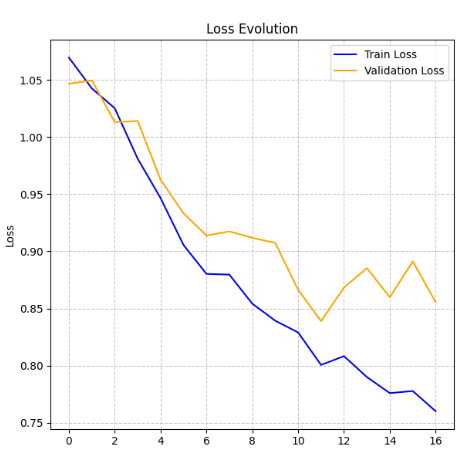
\includegraphics[width=0.75\linewidth]{new figures/Loss.png}
    \caption{Validation Loss  of BiLSTM(Glove)}
    \label{fig:loss}
\end{figure}

Figure \ref{fig:loss} illustrates the loss evolution of the model across 17 training epochs with the patience of 5 epochs. The training loss, represented by the blue line, exhibits a consistent downward trend, indicating effective learning and convergence during training. The validation loss, shown in orange, also decreases overall but displays some fluctuations, particularly in the later epochs (around epoch 12 onward), where it tends to plateau and slightly oscillate which was control by the patience.

\begin{figure}[H]
    \centering
    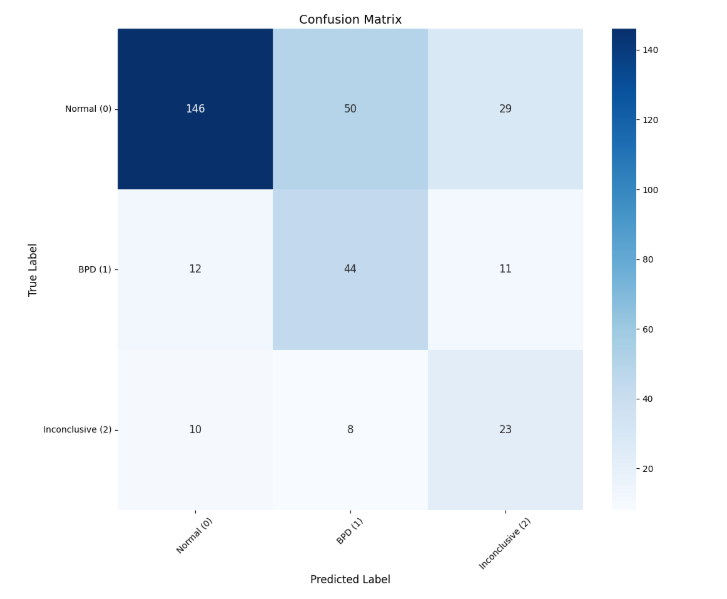
\includegraphics[width=0.90\linewidth]{new figures/Confusion Matrix.png}
    \caption{Confusion Matrix of BiLSTM}
    \label{fig:confusion}
\end{figure}

Figure \ref{fig:confusion} presents the performance of the BiLSTM model after performing text augmentation .  The confusion matrix shows that the model performed best in identifying the Normal class, correctly classifying 146 instances, though it misclassified 50 as BPD and 29 as Inconclusive. For the BPD class, 44 samples are correctly identified, while 12 were incorrectly labeled as Normal and 11 as Inconclusive. The Inconclusive class had the lowest number of correctly classified samples (23), with 10 misclassified as Normal and 8 as BPD.

\vspace{3cm}

\subsection{Comparative Analysis of Large Language Models}

\small
\setlength{\tabcolsep}{10pt}
\renewcommand{\arraystretch}{1.1}
% \begin{center}
\begin{longtable}{lcccc}
\caption{Performance Comparison of Transformer Models on Question-Wise Stratified Split Dataset with No Class Balancing Technique}
\label{tab:transformer_no_balancing} \\
\hline
Model & Accuracy & Precision & Recall & F1 Score \\
\hline
\endfirsthead

\multicolumn{5}{c}%
{{\bfseries Table \thetable\ -- continued from previous page}} \\
% \hline
% \textbf{Models and \newline Feature Extractions} & \textbf{Accuracy} & \textbf{Precision} & \textbf{Recall} & \textbf{F1-score} \\
\hline
\endhead

\hline \multicolumn{5}{r}{{Continued on next page}} 
\endfoot

\hline
\endlastfoot

\textbf{ELECTRA} & \textbf{0.8649} & \textbf{0.8684} & \textbf{0.8649} & \textbf{0.8620} \\
BERT & 0.8168  & 0.8077 & 0.8168 & 0.8092 \\
DistilBERT & 0.8108  & 0.8123 & 0.8108 & 0.8096 \\
RoBERTa & 0.8318 & 0.8432 & 0.8318 & 0.8353 \\
XLNet & 0.8258 & 0.8363 & 0.8258 & 0.8160\\
DeBERTa & 0.8348 & 0.8508 & 0.8348 & 0.8375\\

\end{longtable}
% \end{center}

\vspace{-\baselineskip}
\vspace{0.8em}

\noindent
In \ref{tab:transformer_no_balancing} the transformer models demonstrate superior performance compared to traditional deep learning approaches, with ELECTRA achieving the highest accuracy (0.8649) and F1-score (0.8620) without any class balancing techniques. This suggests that transformer architectures are particularly well-suited for this task.

\small
\setlength{\tabcolsep}{10pt}
\renewcommand{\arraystretch}{1.1}
% \begin{center}
\begin{longtable}{lcccc}
\caption{Performance Comparison of Transformer Models with Inverse Class-Weighted Cross Entropy Loss}
\label{tab:transformer_cwl} \\
\hline
Model & Accuracy & Precision & Recall & F1 Score \\
\hline
\endfirsthead

\multicolumn{5}{c}%
{{\bfseries Table \thetable\ -- continued from previous page}} \\
% \hline
% \textbf{Models and \newline Feature Extractions} & \textbf{Accuracy} & \textbf{Precision} & \textbf{Recall} & \textbf{F1-score} \\
\hline
\endhead

\hline \multicolumn{5}{r}{{Continued on next page}} 
\endfoot

\hline
\endlastfoot

\textbf{ELECTRA} & \textbf{0.8679} & \textbf{0.8698} & \textbf{0.8679} & \textbf{0.8676} \\
BERT & 0.8108  & 0.8170 & 0.8108 & 0.8133 \\
DistilBERT & 0.8108  & 0.8157 & 0.8108 & 0.8126 \\
RoBERTa & 0.8559 & 0.8674 & 0.8559 & 0.8586 \\
XLNet & 0.8168 & 0.8315 & 0.8168 & 0.8203\\
DeBERTa & 0.8438 & 0.8571 & 0.8438 & 0.8446\\

\end{longtable}
% \end{center}

\vspace{-\baselineskip}
\vspace{0.8em}


\noindent
Table \ref{tab:transformer_cwl} shows ,  when applying inverse class-weighted cross entropy loss, ELECTRA maintains its lead with a slight improvement in all metrics (accuracy: 0.8679, F1: 0.8676), while RoBERTa shows the most significant improvement among the other models, suggesting it benefits particularly from this class balancing approach.

\small
\setlength{\tabcolsep}{10pt}
\renewcommand{\arraystretch}{1.1}
% \begin{center}
\begin{longtable}{lcccc}
\caption{Performance Comparison of Transformer Models with Text Augmentation}
\label{tab:transformer_augmentation} \\
\hline
Model & Accuracy & Precision & Recall & F1 Score \\
\hline
\endfirsthead

\multicolumn{5}{c}%
{{\textbf{Table \thetable}\ continued from previous page}} \\
% \hline
% \textbf{Models and \newline Feature Extractions} & \textbf{Accuracy} & \textbf{Precision} & \textbf{Recall} & \textbf{F1-score} \\
\hline
\endhead

\hline 
\endfoot

\hline
\endlastfoot

\textbf{ELECTRA} & \textbf{0.8709} & \textbf{0.8683} & \textbf{0.8709} & \textbf{0.8684} \\
BERT & 0.8408  & 0.8471 & 0.8408 & 0.8433 \\
DistilBERT & 0.7808  & 0.8106 & 0.7808 & 0.7884 \\
RoBERTa & 0.8589 & 0.8645 & 0.8589 & 0.8599 \\
XLNet & 0.8348 & 0.8331 & 0.8348 & 0.8325\\
DeBERTa & 0.8649 & 0.8776 & 0.8649 & 0.8646\\

\end{longtable}
% \end{center}

\vspace{-\baselineskip}
\vspace{0.8em}

\noindent
Table \ref{tab:transformer_augmentation} illustrated text augmentation, ELECTRA achieves its highest performance (accuracy: 0.8709, F1: 0.8684), demonstrating that data augmentation techniques can further enhance transformer model performance. Notably, DeBERTa shows competitive results with the highest precision (0.8776) among all configurations.
\begin{figure}[H]
    \centering
    \begin{subfigure}[b]{0.32\linewidth}
        \centering
        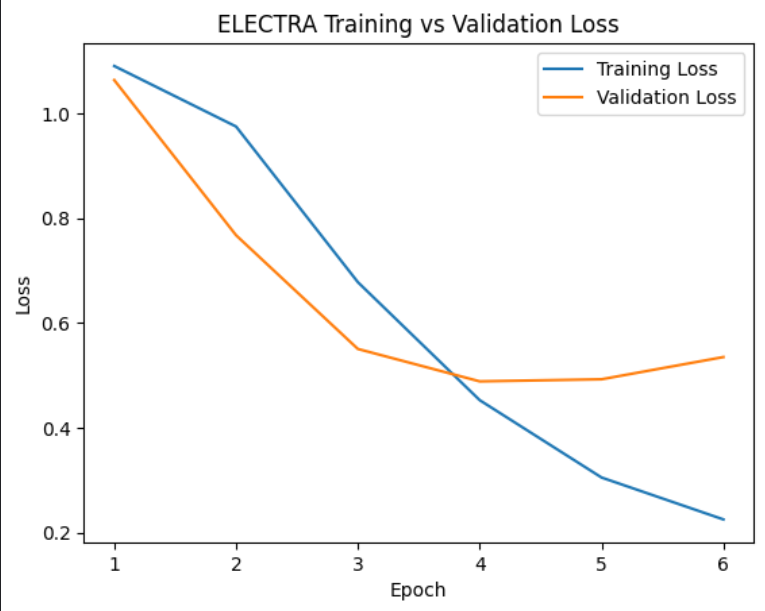
\includegraphics[width=\linewidth]{new figures/ELECTRA (Loss Curves).png}
        \caption{Validation Loss of ELECTRA}
        \label{fig:electra}
    \end{subfigure}
    \hfill
    \begin{subfigure}[b]{0.32\linewidth}
        \centering
        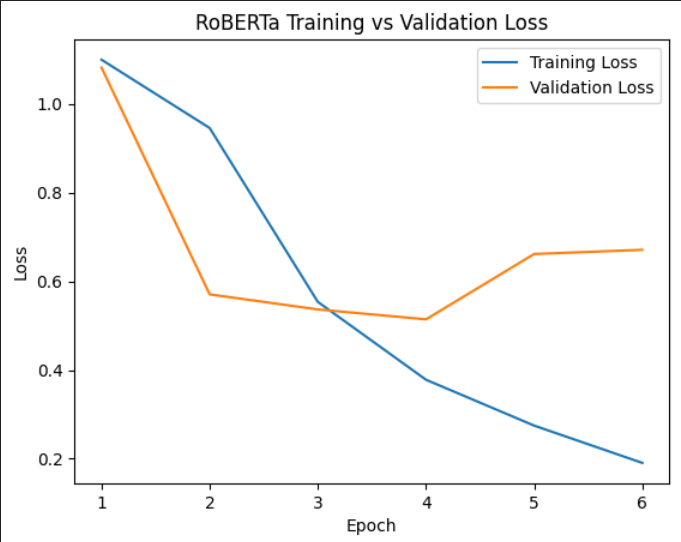
\includegraphics[width=\linewidth]{new figures/RoBERTa (Loss Curves).png}
        \caption{Validation Loss of RoBERTa}
        \label{fig:roberta}
    \end{subfigure}
    \hfill
    \begin{subfigure}[b]{0.32\linewidth}
        \centering
        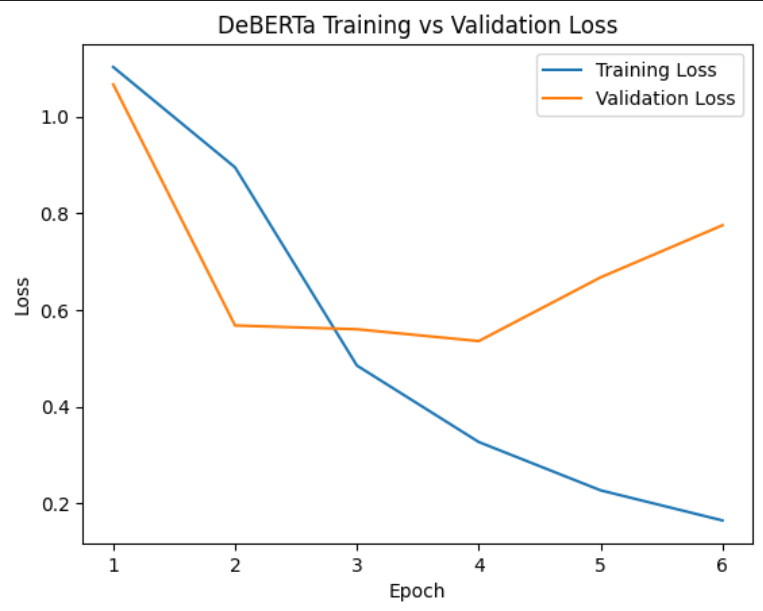
\includegraphics[width=\linewidth]{new figures/DeBERTa (Loss Curves).png}
        \caption{Validation Loss of DeBERTa}
        \label{fig:deberta}
    \end{subfigure}
    \caption{Comparison of validation loss curves for ELECTRA, RoBERTa, and DeBERTa models.}
    \label{fig:loss_comparison}
\end{figure}

 Figure \ref{fig:electra} shows the training and validation losses of the ELECTRA model across 6 epochs. Initially, both losses decrease steadily, indicating effective learning and generalization. However, starting from epoch 4, the validation loss begins to plateau and then slightly increase, while the training loss continues to drop. This divergence suggests that the model may be starting to overfit the training data after epoch 4, as it learns patterns that don't generalize as well to unseen validation data.
 \begin{figure}[H]
     \centering
     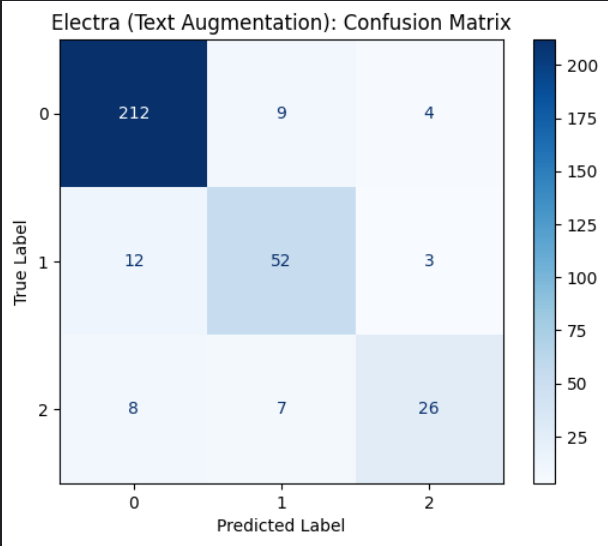
\includegraphics[width=0.5\linewidth]{new figures/ELECTRA (confusion matrix).png}
     \caption{Confusion Matrix of Electra}
     \label{fig:electra_confusion}
 \end{figure}
 
Figure \ref{fig:electra_confusion} illustrates the performance of the ELECTRA model after applying text augmentation on a 3-class classification task. The model correctly predicted class 0 for 212 instances, with only 9 and 4 misclassified as class 1 and class 2, respectively. For class 1, 52 instances were correctly identified, but 12 were misclassified as class 0 and 3 as class 2. Class 2 had 26 correct predictions, with 8 and 7 misclassified as class 0 and class 1, respectively. Overall, the model performs well on class 0 but shows more confusion between classes 1 and 2.
 

\subsection{Stacking Architecture}
Stacking is a powerful ensemble learning method where you train multiple base models and combine their outputs using a meta-model, allowing the system to learn from the strengths and weaknesses of each model.

\begin{figure}[H]
    \centering
    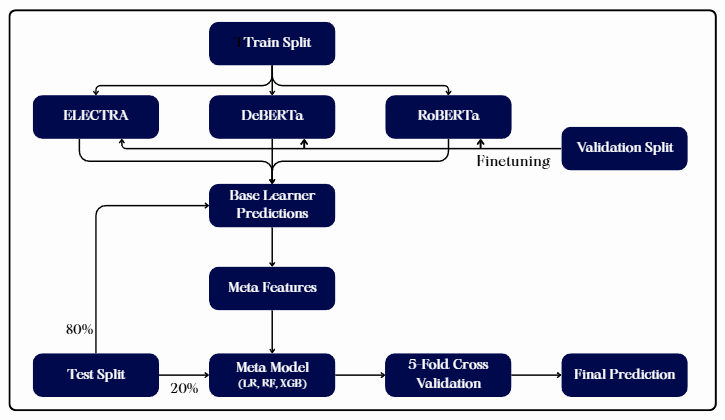
\includegraphics[width=1\linewidth, height=6.25cm]{Stacking Architecture.png}
    \caption{Stacking Architecture}
    \label{fig:stacking_arch}
\end{figure}

In Figure \ref{fig:stacking_arch}, the architecture diagram outlines a multi-stage process where multiple base models were trained and their predictions were combined to generate meta-features. These meta-features were then used to train a final predictive model. The key component of the workflow included some data balancing techniques and rigorous validation through cross-validation to enhance model generalization.

\small
\setlength{\tabcolsep}{4pt}
\renewcommand{\arraystretch}{1.0}
% \begin{center}
\begin{longtable}{lcccc}
\caption{Results of Stacking Architecture with 5 Fold Cross Validation }
\label{tab: stacking_result} \\
\hline
Model & Accuracy & Precision & Recall & F1 Score \\
\hline
\endfirsthead

\multicolumn{5}{c}%
{{\bfseries Table \thetable\ -- continued from previous page}} \\
% \hline
% \textbf{Models and \newline Feature Extractions} & \textbf{Accuracy} & \textbf{Precision} & \textbf{Recall} & \textbf{F1-score} \\
\hline
\endhead

\hline \multicolumn{5}{r}{{Continued on next page}} 
\endfoot

\hline
\endlastfoot

\textbf{Logistic Regression} & \textbf{ $ 0.8645 \pm 0.0466 $ } & \textbf{ $ 0.8718 \pm  0.0441 $} & \textbf{ $ 0.8645 \pm 0.0466 $} & \textbf{$ 0.8628 \pm 0.0414$} \\
Random Forest & $ 0.8616 \pm \ 0.0356 $  & $ 0.8695 \pm 0.0344$ & $ 0.8616 \pm 0.035 6$ & $ 0.8607 \pm 0.0306 $ \\
XGBoost & $ 0.8526 \pm 0.0476 $  & $ 0.8646 \pm 0.0409 $ & $ 0.8526 \pm 0.0476 $ & $ 0.8529 \pm 0.0420 $ \\

\end{longtable}
% \end{center}

\vspace{-\baselineskip}
\vspace{0.8em}


Table \ref{tab: stacking_result} shows results of 5-fold cross-validation using three models, Logistic Regression, Random Forest, XGBoost, as the meta model. Logistic Regression achieved the best performance with an F1-Score of 86.2\%. However, the stacking architecture underperforms compared to the standalone ELECTRA model, which achieved a higher F1-score of 86.84\%.

\subsection{Result Interpretation and Key Findings}
The experimental results highlight several key findings regarding model performance across different techniques. Traditional machine learning models, particularly Linear SVM (LSVM) with TF-IDF demonstrated strong results when combined with oversampling achieving a 70.74\% F1-score with ADASYN outperforming SMOTE’s 66.34\%. Among deep learning models, Bidirectional LSTM with GloVe embeddings (BiLSTM-GloVe) delivered the best performance reaching 63.69\% accuracy and 66.13\% F1-score, underscoring the advantages of bidirectional architectures and contextual word embeddings. However, large language models (ELECTRA, RoBERTa, DeBERTa) significantly outperformed all other approaches, with ELECTRA achieving the highest accuracy (86.49\%) and F1-score (86.20\%) without any class balancing. Further improvements were observed when applying inverse class-weighted loss (86.79\% accuracy, 86.76\% F1-score) and text augmentation (87.09\% accuracy, 86.84\% F1-score), demonstrating the robustness of transformer models in handling imbalanced datasets. Overall, the findings indicate that while traditional and deep learning models benefit from oversampling and feature engineering, transformer architectures particularly ELECTRA with augmentation and weighted loss, deliver the best performance making them the preferred choice for incorporation in the NLP-based screening tool. Compared to the stacking architecture, the standalone ELECTRA model trained on augmented text performs better with a higher F1-score (by a difference of 0.6\%). For this reason, the ELECTRA model, trained on augmented text, was selected as the model for deployment in the NLP-based BPD screening tool.
